\chapter{Unfolding procedure of fake muon control sample}
\label{appx:unfold-tech}

This appendix provides more technical information on step 2--4 in \muon misID
unfolding.

\paragraph{Step 2}
The efficiency \misEff[t]{\hat{t}'}
for a track of true species $t$ satisfying requirements of
a tagged species $\hat{t}'$ is obtained from $t$-enriched \pidcalib samples
which is taken as truth.
Let us first define the subsamples used to evaluate the efficiency,
as shown schematically in \cref{fig:relation-unfolding-sets}:

\begin{itemize}
    \item $t_\text{PIDCalib}$: The $t$-enriched \pidcalib sample itself
        (or MC in the case of ghost).
        The sample contains minimal cuts.
    \item $t_\text{acc}$: The subset of $t_\text{PIDCalib}$ that satisfies all \muon
        cuts other than PID (i.e., track in \muon acceptance).
        Note that this subsample is further divided into two subsamples:
        $t_\text{fake}$ and $\hat{\mu}$.
    \item $t_\text{fake}$: The subset of $t_{acc}$ that \emph{fails} \muon PID
        from \cref{tab:offline-cut-common}.
    \item $\hat{\mu}_t$: The subset of $t_{acc}$ that \emph{passes} \muon PID
    \item $\hat{t}'_\text{fake}$: The subset of $t_\text{fake}$ that passes the
        $\hat{t}'$ tagging requirements
        from \cref{tab:selection-for-tagged-species}.
\end{itemize}

\begin{figure}[ht]
    \centering
    \resizebox{0.8\columnwidth}{!}{
        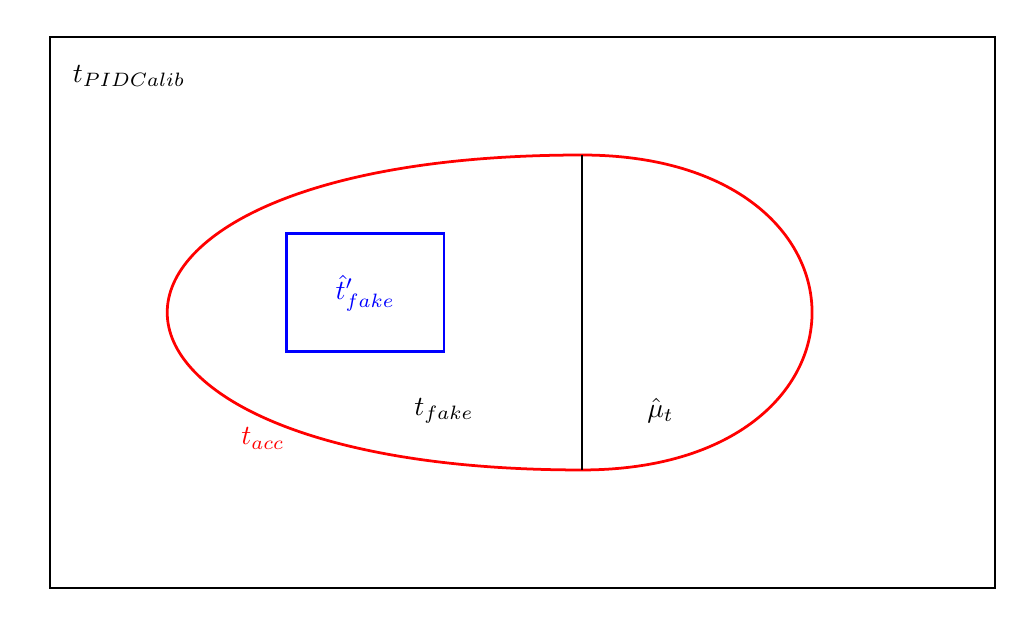
\begin{tikzpicture}
    \pgfdeclarelayer{nodelayer}
    \pgfdeclarelayer{edgelayer}
    \pgfsetlayers{nodelayer,edgelayer}

	\begin{pgfonlayer}{nodelayer}
		\node (0) at (-6, -3.5) {};
		\node (1) at (6, -3.5) {};
		\node (2) at (-6, 3.5) {};
		\node (3) at (6, 3.5) {};
		\node (6) at (-5, 3) {$t_\text{PIDCalib}$};
		\node (7) at (-6, 3) {};
		\node (8) at (-6, -3) {};
		\node (9) at (6, -3) {};
		\node (10) at (6, 3) {};
        \node[red] (11) at (-3.3, -1.6) {$t_\text{acc}$};
		\node (14) at (0.75, -2) {};
		\node (15) at (0.75, 2) {};
		\node (17) at (-1, -1.25) {$t_\text{fake}$};
		\node (18) at (1.75, -1.25) {$\hat{\mu}_t$};
		\node (19) at (-3, 1) {};
		\node (20) at (-3, -0.5) {};
		\node (21) at (-1, -0.5) {};
		\node (22) at (-1, 1) {};
		\node (23) at (-2, 0.25) {};
        \node[blue] (24) at (-2, 0.25) {$\hat{t}'_\text{fake}$};
	\end{pgfonlayer}
	\begin{pgfonlayer}{edgelayer}
        \draw[line width=0.3mm] (1.center)
			 to (0.center)
			 to (2.center)
			 to (3.center)
			 to cycle;
        \draw[red, line width=0.35mm] (15.center)
			 to [in=180, out=180, looseness=4.50] (14.center)
			 to [in=0, out=0, looseness=2.50] cycle;
        \draw[line width=0.3mm] (15.center)
			 to (14.center);
        \draw[blue, line width=0.35mm] (19.center)
			 to (22.center)
			 to (21.center)
			 to (20.center)
			 to cycle;
	\end{pgfonlayer}
\end{tikzpicture}

    }
    \caption{Subsamples of $t$-enriched \pidcalib samples used in unfolding.}
    \label{fig:relation-unfolding-sets}
\end{figure}


The efficiency \misEff[t]{\hat{t}'} of a true $t$ to be classified as $\hat{t}'$
can be computed as:

\begin{equation}
    \misEff[t]{\hat{t}'} =
    \misEff[t^{\phantom{}}_\text{fake}]{\hat{t}'_\text{fake}} = \frac{n_{\hat{t}'_\text{fake}}}{n_{t_\text{fake}}}
\end{equation}
where $n$ denote yields in the \pidcalib \emph{fake} subsamples as shown
in \cref{fig:relation-unfolding-sets}.
All efficiencies are binned in $p_B$, $\eta_B$, and nTracks with a consistent
binning scheme.


\paragraph{Step 3}
In a particular $p_B$-$\eta_B$-nTracks bin,
the measured yields $\tilde{n}_{\hat{t}'}$,
the true yields $\tilde{n}_{t}$,
and the response matrix $M$ have the following relation:

\begin{equation}
    \begin{pmatrix*}[l]
        \tilde{n}_{\hat{\pi}} \\
        \tilde{n}_{\hat{K}}   \\
        \tilde{n}_{\hat{p}}   \\
        \tilde{n}_{\hat{e}}   \\
        \tilde{n}_{\hat{g}}   \\
    \end{pmatrix*}
    =
    \begin{pmatrix*}[l]
        \misEff[\pi]{\hat{\pi}} & \misEff[K]{\hat{\pi}} & \misEff[p]{\hat{\pi}} & \misEff[e]{\hat{\pi}} & \misEff[g]{\hat{\pi}} \\
        \misEff[\pi]{\hat{K}}   & \misEff[K]{\hat{K}}   & \misEff[p]{\hat{K}}   & \misEff[e]{\hat{K}}   & \misEff[g]{\hat{K}}   \\
        \misEff[\pi]{\hat{p}}   & \misEff[K]{\hat{p}}   & \misEff[p]{\hat{p}}   & \misEff[e]{\hat{p}}   & \misEff[g]{\hat{p}}   \\
        \misEff[\pi]{\hat{e}}   & \misEff[K]{\hat{e}}   & \misEff[p]{\hat{e}}   & \misEff[e]{\hat{e}}   & \misEff[g]{\hat{e}}   \\
        \misEff[\pi]{\hat{g}}   & \misEff[K]{\hat{g}}   & \misEff[p]{\hat{g}}   & \misEff[e]{\hat{g}}   & \misEff[g]{\hat{g}}   \\
    \end{pmatrix*}
    \begin{pmatrix*}[l]
        \tilde{n}_{{\pi}} \\
        \tilde{n}_{{K}}   \\
        \tilde{n}_{{p}}   \\
        \tilde{n}_{{e}}   \\
        \tilde{n}_{{g}}   \\
    \end{pmatrix*}
\end{equation}
where $\tilde{n}$ denote yields in the fake \muon control sample
as described in \cref{ref:sel:data:fake-mu},
and \misEff[t]{\hat{t}'} are obtained from step-2.

The Bayesian (iterative) unfolding method provided by \RooUnfold\ is used to
obtain the true yields $\tilde{n}_t$.
At this stage, there is no guarantee that
$\sum_t \tilde{n}_t = \sum_{\hat{t}'} \tilde{n}_{\hat{t}'}$.
Naive matrix inversion cannot be used because it is sensitive to statistical
fluctuations.  % TODO: Should I cite Cowan here?

To find \misEff[\hat{t}']{t}, recall its definition:

\begin{equation}
    \misEff[\hat{t}']{t^{\phantom{}}} \equiv
        \frac{
            \text{Number of $\hat{t}'$-tagged tracks from true $t$ tracks}
        }{
            \text{Total number of $\hat{t}'$-tagged tracks based on unfolding}
        }
\end{equation}

With the unfolded true yields, we can compute:

\begin{itemize}
    \item Number of $\hat{t}'$-tagged tracks in true $t$ tracks:
        $\tilde{n}_t \cdot \misEff[t]{\hat{t}'}$.
    \item Total number of $\hat{t}'$-tagged tracks based on unfolding:
        $\sum_t \tilde{n}_t \cdot \misEff[t]{\hat{t}'}$.
        The definition used here ensures the total number of tracks is
        conserved by unfolding.
\end{itemize}

Put them together:

\begin{equation}
    \misEff[\hat{t}']{t^{\phantom{}}} =
        \frac{
            \tilde{n}_t \cdot \misEff[t^{\phantom{}}]{\hat{t}'}
        }{
            \sum_t \tilde{n}_t \cdot \misEff[t^{\phantom{}}]{\hat{t}'}
        }
\end{equation}

\paragraph{Step 4}
To obtain \misEff[\hat{t}']{\hat{\mu}},
what is really needed is:
$\misEff[\hat{t}']{t_\text{acc}} \cdot \misEff[t_\text{acc}]{\hat{\mu}}$.
However, \misEff[\hat{t}']{t} is obtained with \emph{fake} \muon control
samples, which is directly comparable to $t_\text{fake}$ subsample in
\cref{fig:relation-unfolding-sets}.
It is assumed that:

\begin{equation}
    \misEff[\hat{t}']{t_\text{acc}} =
    \frac{
        \misEff[\hat{t}']{t}
    }{
        \misEff[t_\text{acc}]{t}
    } \approx
    \frac{
        \misEff[\hat{t}']{t}
    }{
        \misEff[t_\text{acc}]{t_\text{fake}}
    }
\end{equation}
note that the nominator uses $t/t'$ as labels to species, whereas the
denominator uses $t_\text{acc}/t_\text{fake}$ as labels to subsamples
in the $t$-enriched \pidcalib sample.
This is unfortunate but clearer notations can be much more verbose.
